\documentclass[12pt]{article}
\linespread{1.465}

\usepackage{amsmath}
\usepackage{multicol}
\usepackage{graphicx}

%\documentstyle[11pt]{article}

\setlength{\topmargin}{-.5in}
\setlength{\textheight}{9in}
\setlength{\oddsidemargin}{.125in}
\setlength{\textwidth}{6.25in}


\begin{document}

%\noindent
\setlength{\parindent}{24pt}


\section*{Project 1 - Matrix Multiplication}
Team 27 \--- David Eckman, Bryce Evans, Batu Inal

\section{Motivation}

Our assignment was to enhance the performance (GFlops/s) of matrix multiplication ($C = AB$ for $M \times M$ square matrices) by improving arithmetic intensity, memory access, and cache efficiency.
In our analysis, we considered five main modifications: (1) changing the order of loops for matrix multiplication both within and among blocks; (2) using the restrict keyword to achieve strong optimizations by the compiler, (3) using different compiler flags, (4) changing the block size relative to cache, (5) copying and restructuring matrices in memory, and combinations thereof.

\section{Methods}

\subsection{Changing the Order of Loops}

The basic matrix multiplication algorithm uses three nested loops to determine the order of updates.
We tested all six orderings of the loops for complete verification. 
Figure \ref{fig:LoopOrders} shows the performance of the orderings for the basic algorithm.

We observed that the performances of the loop orders were consistently paired by which index was in the inner loop.
Orderings with index $j$ in the inner loop performed the worst while orderings with index i in the inner loop performed far better.
The reason for the performance differences among these ordering has to do with the memory access patterns they create and how that agrees with the storage of the matrices in memory.
The access patterns of the different orderings can be visualized by considering the update formula $c_{i,j} \mathrel{+}= a_{i,k} \times b_{k,j}$, or as it appears in the code:
\begin{verbatim} C[j*lda+i] = A[k*lda+i] * B[j*lda+k];\end{verbatim}

\begin{center}
\begin{figure}[h]
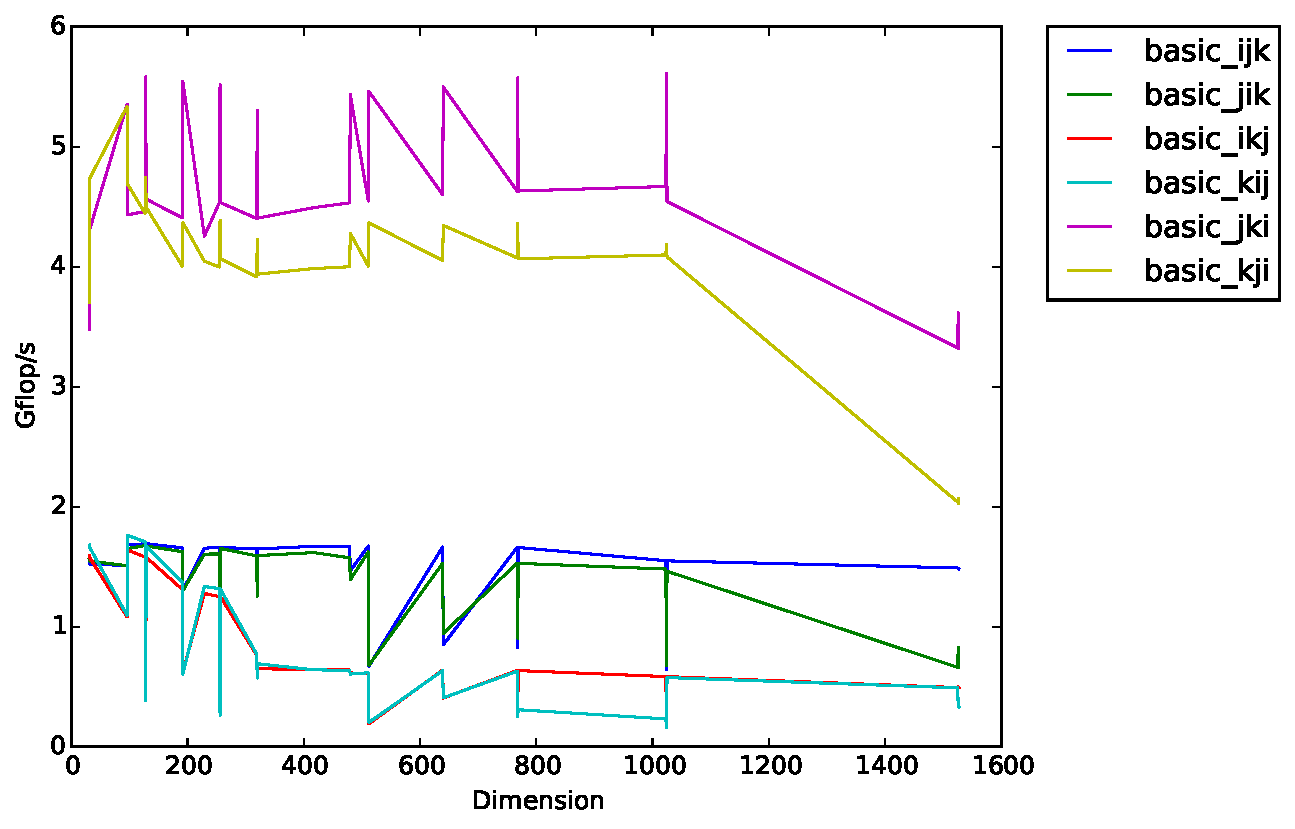
\includegraphics[width=6in]{timing_basiclooporders_comparison.pdf}
	\caption{Performance for various loop orders.}
	\label{fig:LoopOrders}
\end{figure}
\end{center}

By putting $i$ in the innermost loop, we fix the element $k,j$ of \texttt{B} and pass through column $j$ of $C$ and column $k$ of $A$.
This access pattern is the most favorable because the matrices $A$, $B$, and $C$ are stored in memory in column major form.
This arrangement would then allow us to keep part or all of a column of a matrix in cache instead of reloading it.

Alternatively, when $j$ is in the innermost loop, we would fix the $i,k$ element of $A$ and pass through row $i$ of $C$ and row $k$ of $B$.
This would be the least desirable access pattern and the performance in Figure \ref{fig:LoopOrders} reflects this.

To distinguish between $jki$ and $kji$, note that by putting $k$ in the middle loop, we switch the column of $C$ less frequently---only in the outer loop.
Figure \ref{fig:LoopOrders} shows that the loop order $jki$ performs the best.
In the block matrix multiplication algorithms we test later, we chose to use the $jki$ loop ordering both within and among the blocks.

\subsection{Restrict Keyword}

The \texttt{restrict} keyword allows the compiler to perform strong optimizations.
By using \texttt{restrict}, we tell the compiler that pointers will be unique and only accessed directly.
This allows optimization by eliminating the need to reload values repeatedly after updates.
%Consider the case of loading a pointer $A$ and adding it to a value at pointer $B$ and pointer $C$.
%Without using \texttt{restrict}, $A$ would need to be reloaded after updating $B$ because $A$ and $B$ could be the same value.
%With \texttt{restrict}, we only load $A$ once, which is appropriate for our usage because we can guarantee that no value in a matrix is ever used to update itself. 
Figure \ref{fig:Restrict} shows the potential speedup offered by \texttt{restrict} when applied to the basic matrix multiplication algorithm with $ijk$ loop ordering.
An interesting observation is that the lowest performance points without \texttt{restrict} (often when the dimension $M$ is a power of two) are the best performance points with \texttt{restrict}.
We suspect this result is a factor of the cache associativity, but we do not have a clear intuition.

\begin{center}
\begin{figure}[h]
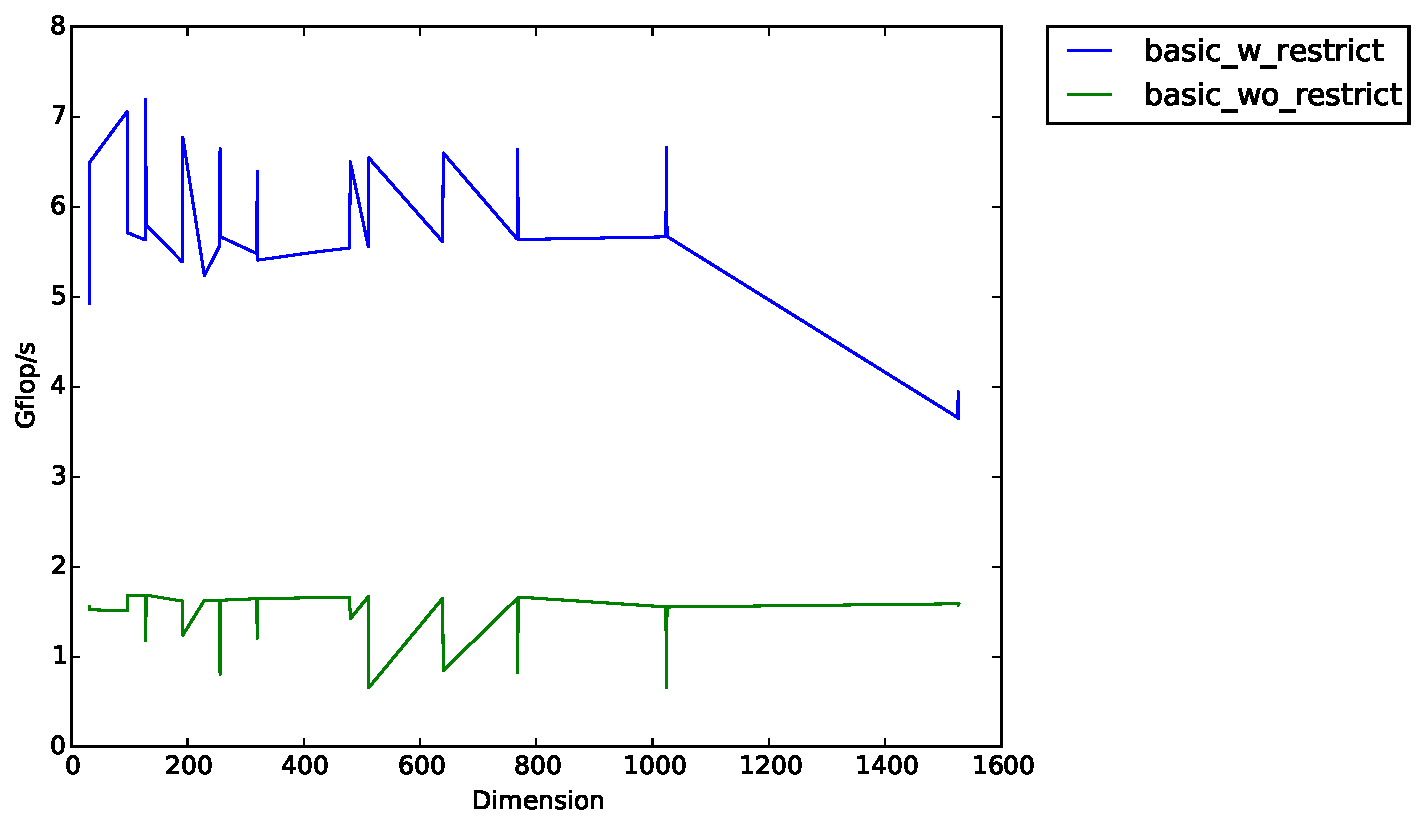
\includegraphics[width=6in]{timing_basic_ijk_w_wo_restrict_comparison.pdf}
	\caption{Performance with and without \texttt{restrict}.}
	\label{fig:Restrict}
\end{figure}
\end{center}

\subsection{Compiler Flags}

We tried an array of compiler flags for optimizing code.
We targeted flags that improved performance in terms of faster code execution, as opposed to code size, compilation time, or memory usage.
We list below the flags we tested:

\begin{multicols}{3}
\begin{verbatim}
-O3 
-opt-prefetch 
-unroll-aggressive
-ansi-alias 
-ftree-vectorize 
-xHost 
-axCORE-AVX2 
-qopt-report-phase=vec
\end{verbatim}
\end{multicols}

The flag \texttt{-O3} adds significant optimizations across the board, taking more compile time but interchanging order of operations for improved speeds as well as some loop unrolling (also assisted by \texttt{-unroll-aggressive}).
Because our application uses many floating point operations in loops, this is a strong option to increase speed.
Using \texttt{-O3} in another application could potentially slow down code execution.

Matrix multiplication does a similar operation many times across many data. We use prefetching (with \texttt{-opt-prefetch}) to load data into memory without halting execution. We had these ideas suggested to us from gh:\texttt{kenlimmj}.

We also used the flag \texttt{-qopt-report-phase=vec} to produce vectorization reports from icc and identify areas for improvement.

The remainder of the flags (\texttt{-ansi-alias, -ftree-vectorize, -xHost,
-axCORE-AVX2}) include a series of options to utilize AVX (Advanced Vector Extensions) and SIMD operations (Single Instruction, Multiple Data).
These add vectorization operations are able to use a single core to load two doubles side by side for processing.
Ignoring overhead, this allows to potentially achieve twice the performance as without such operations. 

Figure \ref{fig:Flags} shows the performance improvements achieved by using these compiler flags when applied to the basic matrix multiplication algorithm with loop order $ijk$.

\subsection{Block Size Relative to Cache Size}

We also explored the approach of partitioning the matrices into smaller matrices (blocks) and multiplying them.
By using this approach we aimed to improve our arithmetic intensity by performing many multiplication operations with the same data.
We also aimed to improve our memory access patterns by choosing the block size so that a block each from matrices $A$, $B$, and $C$ could fit into our L1 or L2 cache.

\begin{center}
\begin{figure}[h]
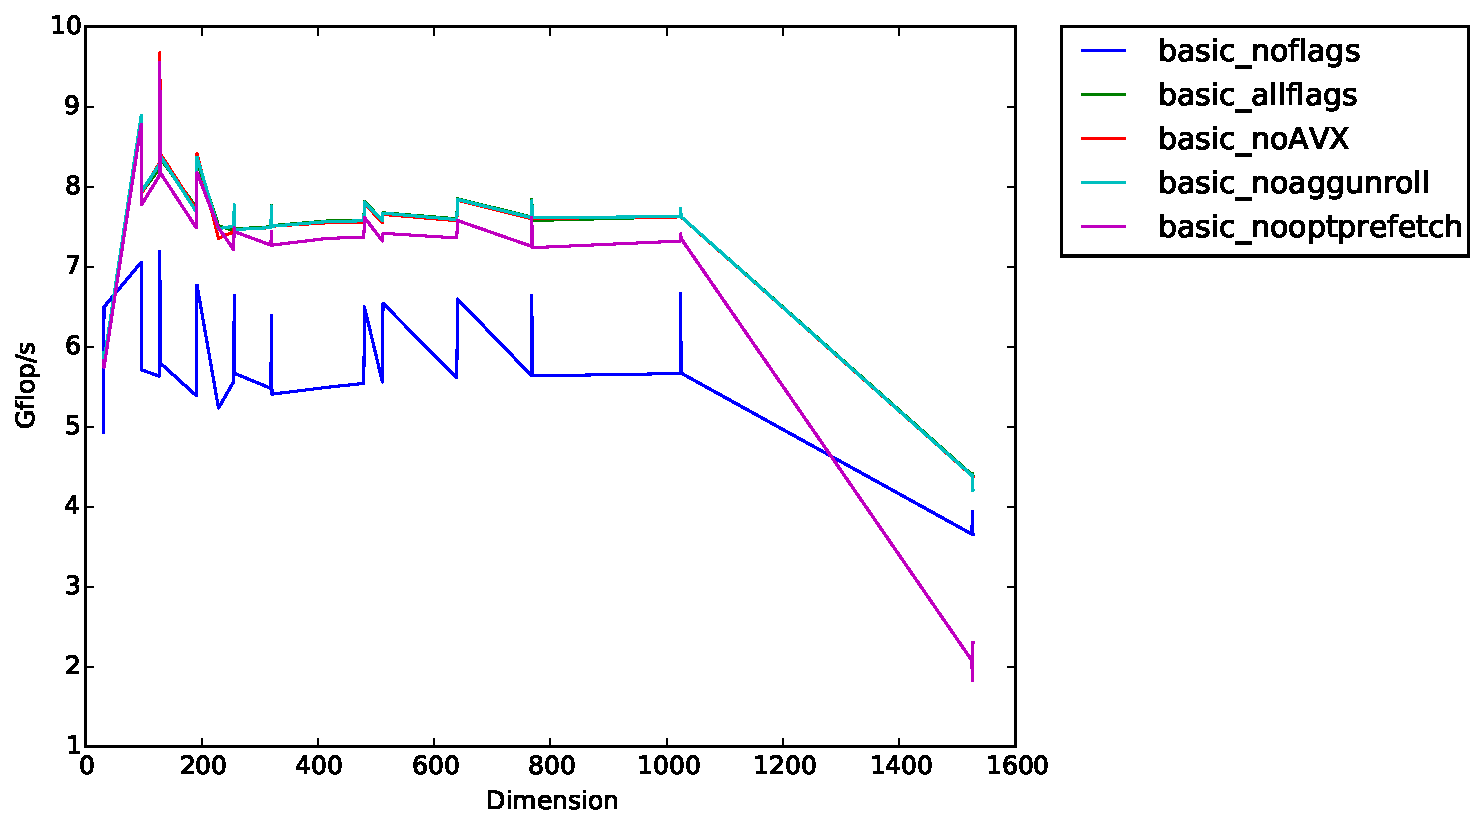
\includegraphics[width=6in]{timing_basic_ijk_flags_comparison.pdf}
	\caption{Performance with different flag settings.}
	\label{fig:Flags}
\end{figure}
\end{center}



On the compute nodes of the totient cluster, L1 cache was 32KB 8-way set-associative, L2 cache was 256 KB 8-way set-associative and L3 was 15MB (shared) 20-way set-associative.
Our initial approach was to utilize the L1 cache without regarding the L2 or the L3 cache. Our calculations for the block size required in order to fit three blocks into L1 cache was as follows:

\begin{align*}
32\text{KB} * 1024\text{B}/\text{KB} * 1 \text{ double}/8\text{B} &= 4096 \text{doubles}\\
4096 \text{ doubles}/ 3 \text{ matrices} &\approx 1365 \text{ doubles}/\text{matrix}.
\end{align*}
Since there are $N^2$ values in a matrix: \[\text{Max block size} = \lfloor{\sqrt{1365}}\rfloor = 36 .\]

We predicted that the overhead of going to the L2 cache if there was a miss in L1 cache would be very low. Therefore we made the exact same calculations for fitting three blocks in the L2 cache.
The calculated maximum block size was 104.

We testing a range of block sizes, most of them a power of two, however we did not observe any remarkable performance for block sizes of 36 and 104.
Figure \ref{fig:BlockSizes} shows the performance of the blocked matrix algorithm for loop order $jki$ at different block sizes.

\begin{center}
\begin{figure}[h]
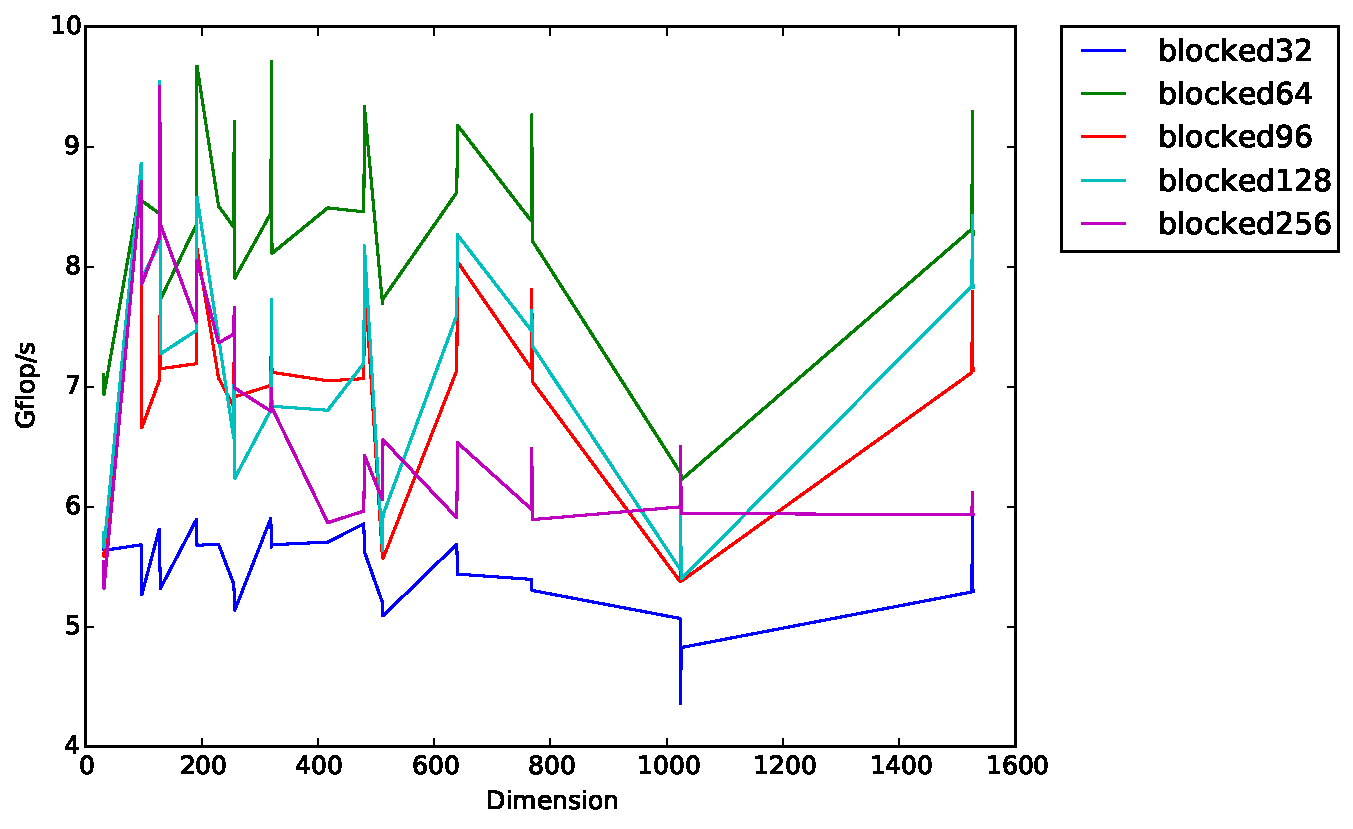
\includegraphics[width=6in]{timing_blocked_comparison.pdf}
	\caption{Performance with various block sizes.}
	\label{fig:BlockSizes}
\end{figure}
\end{center}

Figure \ref{fig:BlockSizes} suggests that a block size of 64 is be the most favorable blocksize of those tested.
A worthwhile observation from the graph is that over all block sizes, the block matrix algorithm suffers poor performance around dimension 1024.
We again believe this trend is due to the associativity of the caches.
To improve the performance for large dimensions, we explored copy optimization.

\subsection{Copy Optimization}

Another method we attempted was to copy the matrices $A$, $B$, and $C$ into memory to improve memory access patterns during the block multiplication operations.
More precisely, we restructured the matrices so that the elements of each block were stored in contiguous memory in column major form.
The order of the blocks in memory also followed column major form.
We chose column major form within and among the blocks of the new matrices because of the ordering of the loops; with the index $i$ in the inner loop, matrices $C$ and A are accessed vertically.
We believed that the improved access patterns in the block-block multiplications would outweigh the computational overhead of copying the matrices.
We managed to write the copy optimization code to avoid padding with zeros so that we could multiply blocks that were not square.
To tune the copy optimization implementation, we also tested a range of block sizes, as shown in Figure \ref{fig:CopyBlockSizes}.  

\begin{center}
\begin{figure}[h]
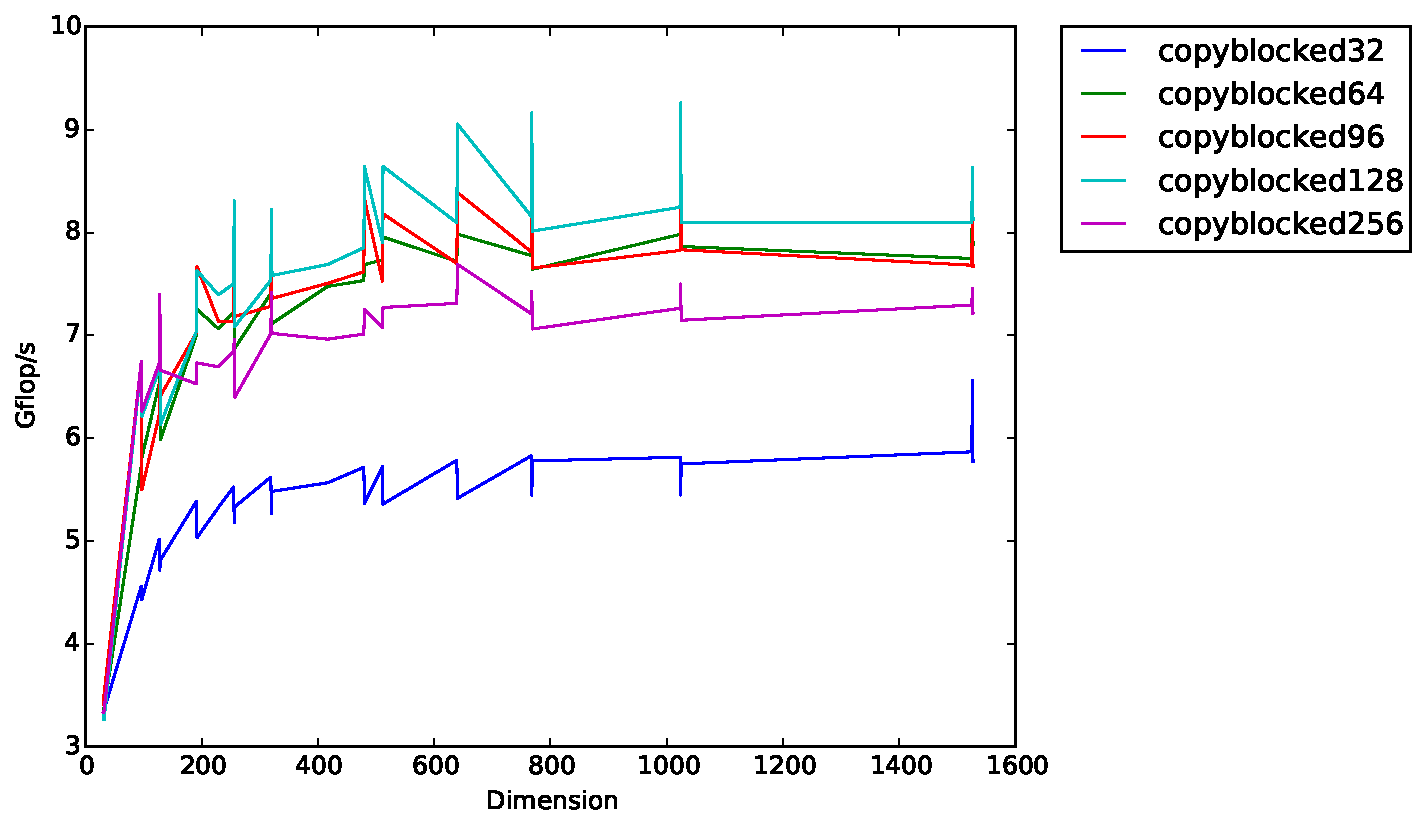
\includegraphics[width=16cm]{timing_copyblocked_comparison.pdf}
	\caption{Performance for CopyOpt + Block for various block sizes.}
	\label{fig:CopyBlockSizes}
\end{figure}
\end{center}



Based on the results shown in Figure \ref{fig:CopyBlockSizes}, we decided to more closely examine block size between 96 and 128.
We chose to test block sizes in this range which were multiples of 8 because that is the number of doubles that fit in a 64-byte register.
From the results in Figure \ref{fig:CopyBlockSizesZoom}, the block sizes of 112 and 120 showed high performance.
We could not think of a reason why these block sizes would be superior to 96 or 128 and we were not able to replicate the results during later testing.

\begin{center}
\begin{figure}[h]
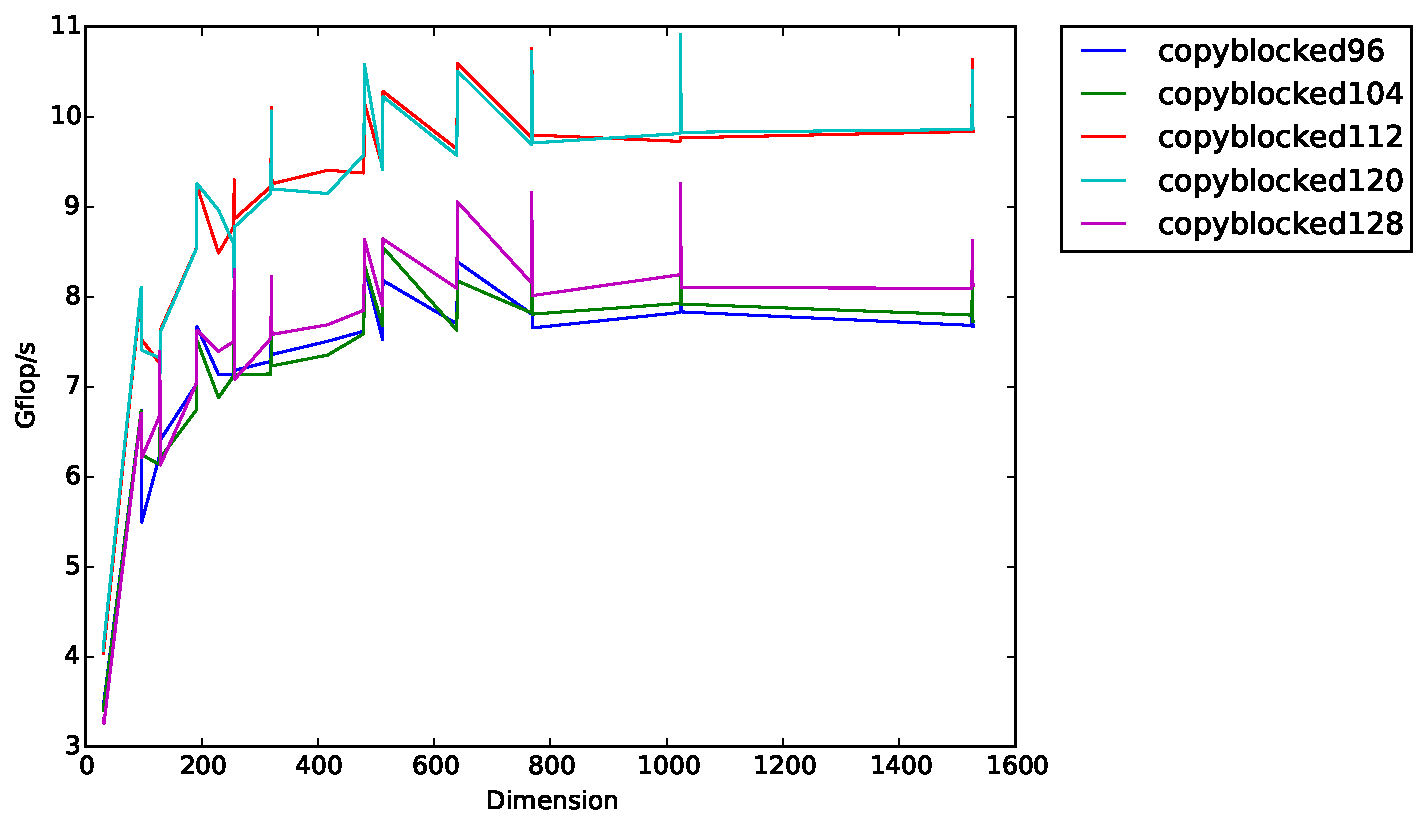
\includegraphics[width=16cm]{timing_copyblocked_comparison_zoom.pdf}
	\caption{Performance for CopyOpt + Block for various block sizes.}
	\label{fig:CopyBlockSizesZoom}
\end{figure}
\end{center}

As shown in Figures \ref{fig:CopyBlockSizes} and \ref{fig:CopyBlockSizesZoom}, we observed a general trend of improving performance as the dimension of the matrices increased.
This can be explained by the fixed overhead involved with copying the matrices.
For this reason, it would not be beneficial for small sized matrices.
In particular, we noticed that the cost of copying was amortized in big matrices, of around $M>200$.
We therefore decided to copy the matrices that were over the threshold of 200 and leave them as is, if they were less than the determined threshold of 200.
In Figure \ref{fig:BestBlas} we show how competitive our best algorithm was to BLAS.

\section{Failed Methods and Future Ideas}
We tried a number of methods that did not result in higher performance, namely manual loop unrolling, multi-level blocking, GCC compilation and flags, and a brief attempt to implement sub-cubic multiplication. 

\begin{center}
\begin{figure}[h]
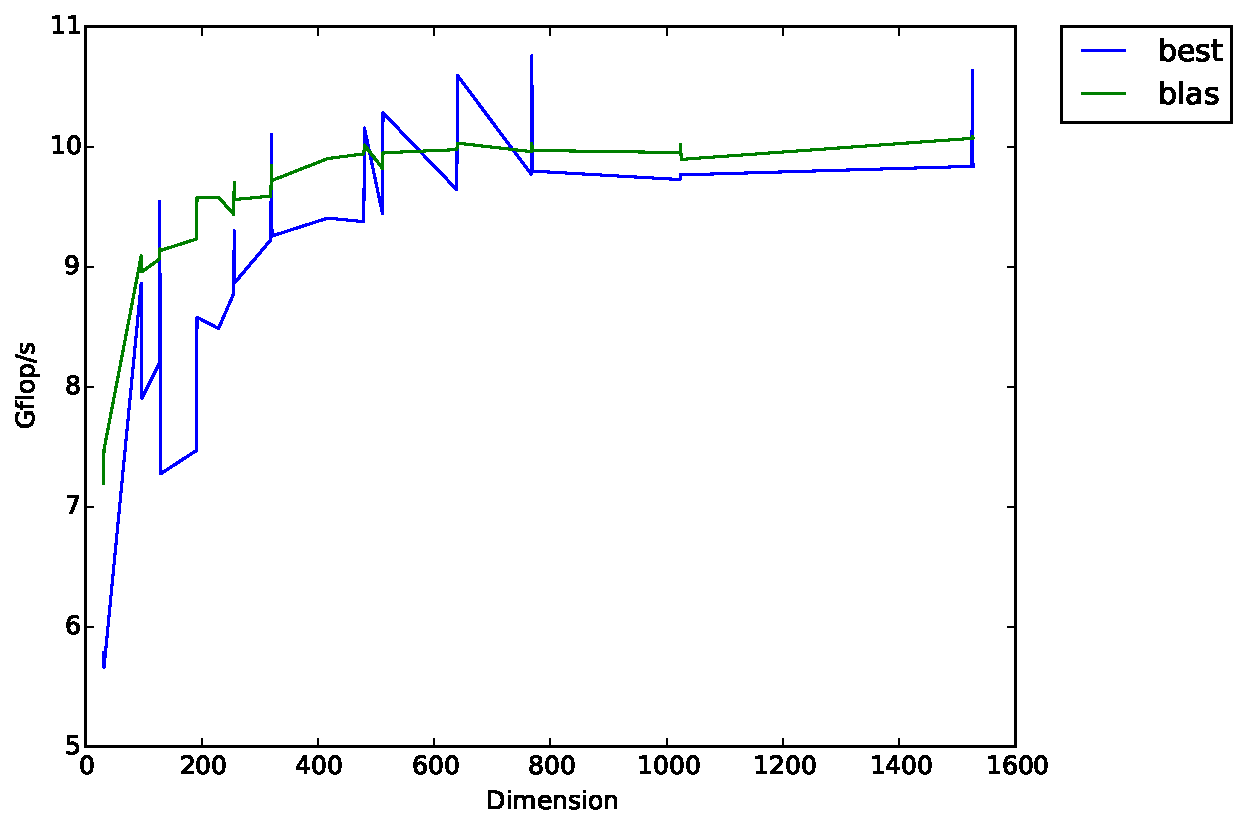
\includegraphics[width=16cm]{timing_blas_vs_best.pdf}
	\caption{Performance of best method vs BLAS.}
	\label{fig:BestBlas}
\end{figure}
\end{center}

Manual loop unrolling, even across various variables or orders of loops, was not as effective as the compiler unrolling.
This was a surprise because other groups in the class (gh: \texttt{sheroze1123}) included this in their implementation and found it to beneficial.
We believe that in our attempts, the compiler no longer optimized these sections despite those optimizations being superior to ours.

Our preliminary attempts at multi-level blocking based on L1 and L2 cache sizes gave poor performance.
Given more time, we would attempt this again with better testing of multi-level block sizes to optimize for architecture.
We attempted to implement the multi-level blocking scheme with copy optimization, but struggled with the coding since the non-padding zeros method involved many oddly-sized or oddly-indexed blocks.

With our attempts at gcc compilation, while much more documentation is available for gcc, the vectorization and parallel support was lacking. ICC was far superior with these benefits, giving great performance increases with a few flags and ease of enabling vectorized operations. 

Lastly, we explored alternative methods to do sub-cubic matrix multiplication, but it was quickly apparent that the large overhead and pre-computations would dominate the actual time the program would run. If we were to run this program across very large matrices (e.g. unable to fit on a single machine), this large pre-computation could become advantageous.

One idea that we did not implement but could nonetheless prove worthwhile was to copy the matrix $A$ as its transpose.
Then the $ijk$ loop ordering would involve going down columns of $A$ and $B$.
We saw that the \texttt{restrict} keyword was very successful in improving the performance of the $ijk$ loop ordering and believe it could have a similar impact in this setting.

\section{Summary}

We have discussed several approaches to accelerate the flop rate of matrix multiplication for square matrices.
Our experiments suggests that; changing the loop ordering to $jki$, utilizing the compiler optimizations such as AVX (Advanced Vector Extensions) and SIMD operations (Single Instruction, Multiple Data), using the \texttt{restrict} keyword to ensure that pointers will be unique and only accessed directly, determining an optimal block size of 112/120, and finally copying the matrices into memory if the size of matrices is greater than 200.
All together, these methods enhanced the performance of the matrix multiplication by almost factor of five compared to the naive implementation.
Further work could be done to debug our failed attempts and try various techniques in current literature such as aligning the memory in order to have more efficient loads into the cache and transposing matrices. 

\subsection{References}

\begin{verbatim}
https://icl.cs.utk.edu/svn/lapack-dev/lapack/trunk/BLAS/SRC/dgemm.f

\end{verbatim}

\end{document}